% !Mode:: "TeX:UTF-8"

\chapter{绪论}

\section{引言}

\subsection{引用参考文献}
引用参考文献示例:在references.bib中添加参考文献对应的bibtex,使用$\backslash$cite\{\}引用论文的id,引用参考文献\cite{barnes2009patchmatch}。

\subsection{插入图片}
如图\ref{fig:figure1}所示,为在文章中插入图片的示例:在latex中使用$\backslash$begin\{figure\}插入图片,支持的格式有jpg、png、eps与pdf等;使用$\backslash$begin\{tabular\}插入三幅图像(一行三列),如果只插入一副图像则不需要使用$\backslash$begin\{tabular\}。

\begin{figure}[htb]
	\centering
	\setlength\tabcolsep{3pt}  % 同一行中的图片间隔
	\vspace{5pt} % 图片上部的空白,如果太小的话,图片顶部会与正文内容十分接近
	\begin{tabular}{ccc}
		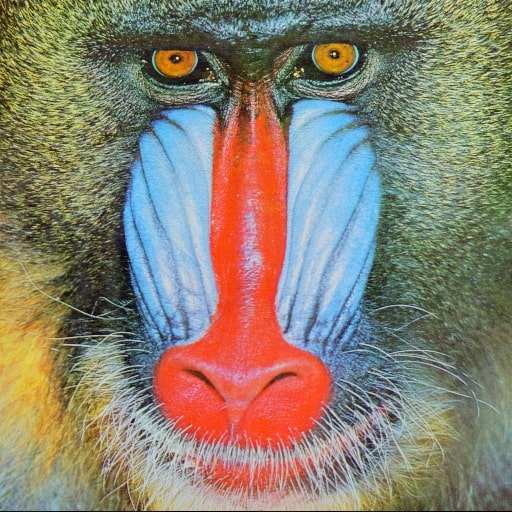
\includegraphics[width=0.32\textwidth]{baboon.jpg} &
		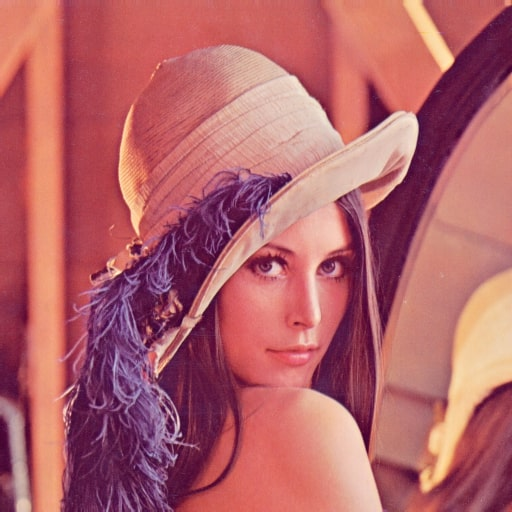
\includegraphics[width=0.32\textwidth]{lena.jpg} &
		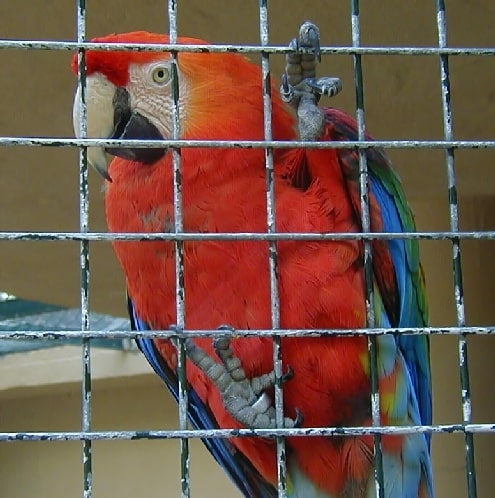
\includegraphics[width=0.32\textwidth]{parrot.jpg} \\
		(a) 图1 & (b) 图2 & (c) 图3 \\[1ex]
	\end{tabular}
	\caption{图片示例}
	\label{fig:figure1}
\end{figure}

\subsection{插入公式}
在文章中插入公式示例:
\begin{equation}
	c = a + b
	\label{eq:equation1}
\end{equation}

\subsection{插入表格}

如表格\ref{tb:table1}所示,为在文章中插入表格的示例。可以通过latex表格在线创建网站(https://www.tablesgenerator.com/),通过用户界面形式创建表格,并转化为latex代码。

\begin{table}[]
	\caption{表格标题}
	\label{tb:table1}
	\centering
	\begin{tabular}{|c|c|c|}
		\hline
		a   & b   & c   \\ \hline
		1.1 & 1.2 & 1.3 \\ \hline
		1.4 & 1.5 & 1.6 \\ \hline
	\end{tabular}
\end{table}

\section{本文思路及研究方法}

本文思路及研究内容

\section{论文结构}

论文结构




